\documentclass[12pt]{article}
\usepackage[a4paper,margin=1in]{geometry}
\usepackage{amsmath, amssymb}
\usepackage{graphicx}
\usepackage{tikz}
\usepackage{caption}
\usepackage{float}
\usepackage{fancyhdr}
\pagestyle{fancy}
\fancyhead[L]{}
\fancyhead[C]{\textbf{Numerical Solution of 1D Viscous Burgers' Equation}}
\fancyhead[R]{}
\setlength{\headheight}{15pt}

\title{\textbf{Numerical Solution of the 1D Viscous Burgers' Equation\\ Using Finite Volume Godunov Scheme}}
\author{}
\date{}

\begin{document}
\maketitle

\section*{1. Introduction}
The 1D viscous Burgers’ equation is a prototype model used in fluid dynamics that combines nonlinear convection and viscous diffusion. While relatively simple in form, it exhibits rich behaviors such as shock formation, wave propagation, and smoothening due to viscosity. This makes it an excellent test problem for numerical methods.

We implement a **finite volume scheme** using:
\begin{itemize}
    \item \textbf{Godunov flux} for accurate nonlinear convection handling,
    \item \textbf{Central difference} for spatial diffusion discretization,
    \item \textbf{Explicit Euler} for time stepping under CFL constraints.
\end{itemize}

\section*{2. Why This Approach?}
\begin{itemize}
    \item \textbf{FVM is conservative:} Each control volume integrates flux across its boundaries, preserving the quantity.
    \item \textbf{Godunov's method handles shocks naturally:} It selects physically correct fluxes for discontinuous solutions.
    \item \textbf{Central differencing is second-order accurate:} It’s easy to implement and effective for smooth diffusion terms.
    \item \textbf{Explicit time stepping is simple and transparent:} While it has limitations, it’s sufficient and stable under CFL conditions.
\end{itemize}

\section*{3. Problem Definition}
We solve the following partial differential equation:

\[
\frac{\partial u}{\partial t} + u \frac{\partial u}{\partial x} = \nu \frac{\partial^2 u}{\partial x^2}, \quad x \in [0,1],\ t > 0
\]

\textbf{Initial condition (Riemann step):}
\[
u(x, 0) =
\begin{cases}
1, & x \leq 0.5 \\
0, & x > 0.5
\end{cases}
\]

\textbf{Boundary conditions:}
\[
u(0,t) = 1,\quad u(1,t) = 0,\quad \forall t
\]

\section*{4. What is the Burgers’ Equation?}
The viscous Burgers' equation is often used to model 1D flow with both nonlinear advection and viscous diffusion. It can be considered a simplified 1D analog of the Navier–Stokes equation. Its two key components are:
\begin{itemize}
    \item \textbf{Nonlinear convection term: } \( u \frac{\partial u}{\partial x} \) represents self-advection of velocity.
    \item \textbf{Viscous term: } \( \nu \frac{\partial^2 u}{\partial x^2} \) causes diffusion and smoothening.
\end{itemize}

\section*{5. What is a Riemann Step?}
A Riemann problem is an initial value problem with a discontinuous initial condition. In our case:

\[
u(x, 0) = 
\begin{cases}
1, & x \leq 0.5 \\
0, & x > 0.5
\end{cases}
\]

This setup is useful to study how discontinuities evolve — forming either shocks (discontinuities) or rarefaction (smooth waves) over time.

\section*{6. Grid Discretization (Finite Volume)}
We divide the domain \( [0,1] \) into \( N \) uniform control volumes with spacing \( \Delta x \). Each control volume tracks the average value of \( u \) over that interval.

\begin{figure}[H]
\centering
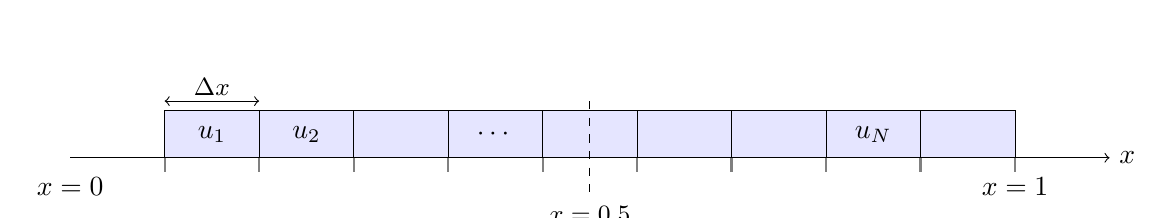
\begin{tikzpicture}[scale=1.2]
  \draw[->] (0,0) -- (11,0) node[right] {$x$};
  \foreach \i in {1,2,...,10}
    \draw[gray, thick] (\i, -0.15) -- (\i, 0.15);
  \foreach \i in {1,2,...,9}
    \draw[fill=blue!10] (\i,0) rectangle (\i+1,0.5);

  \node at (1.5,0.25) {$u_1$};
  \node at (2.5,0.25) {$u_2$};
  \node at (4.5,0.25) {$\cdots$};
  \node at (8.5,0.25) {$u_{N}$};

  \draw[dashed] (5.5,0.6) -- (5.5,-0.4);
  \node at (5.5,-0.6) {\small $x=0.5$};

  \draw[<->] (1,0.6) -- (2,0.6);
  \node at (1.5,0.75) {\small $\Delta x$};

  \node at (0,-0.3) {$x=0$};
  \node at (10,-0.3) {$x=1$};
\end{tikzpicture}
\caption{Finite Volume Grid with cell centers at $x_i$ and size $\Delta x$}
\end{figure}

\section*{7. Numerical Scheme: Detailed Steps}

\subsection*{Step 1: Initial Condition}
Set values according to the Riemann step:
\[
u^0_i =
\begin{cases}
1, & x_i \leq 0.5 \\
0, & x_i > 0.5
\end{cases}
\]

\subsection*{Step 2: Godunov Flux for Nonlinear Convection}
The Godunov method solves the Riemann problem at each interface. For scalar Burgers' equation (convex flux), we simplify it as:

\[
f(u) = \frac{u^2}{2}
\]

\textbf{Interface flux} \( F_{i+1/2} \) is computed as:

\[
F_{i+1/2} = 
\begin{cases}
\frac{1}{2} u_i^2, & \text{if } u_i, u_{i+1} \geq 0 \\
\frac{1}{2} u_{i+1}^2, & \text{if } u_i, u_{i+1} \leq 0 \\
0, & \text{if } u_i < 0 < u_{i+1} \\
\max\left( \frac{1}{2} u_i^2, \frac{1}{2} u_{i+1}^2 \right), & \text{if } u_i > u_{i+1}
\end{cases}
\]

This ensures we select the physically correct flux based on upwinding and entropy conditions.

\subsection*{Step 3: Central Difference for Diffusion}
The second-order derivative \( \frac{\partial^2 u}{\partial x^2} \) is approximated as:

\[
\left( \frac{\partial^2 u}{\partial x^2} \right)_i \approx \frac{u_{i-1} - 2u_i + u_{i+1}}{\Delta x^2}
\]

This uses values from neighboring cells and gives good accuracy for smooth fields.

\subsection*{Step 4: Time Integration (Explicit Euler)}
We use the explicit Euler method:

\[
u_i^{n+1} = u_i^n + \Delta t \left[ -\frac{F_{i+1/2} - F_{i-1/2}}{\Delta x} + \nu \cdot \frac{u_{i-1}^n - 2u_i^n + u_{i+1}^n}{\Delta x^2} \right]
\]

Each term corresponds to physical processes:
\begin{itemize}
    \item Convection handled via flux difference.
    \item Diffusion handled via central difference.
\end{itemize}

\subsection*{Step 5: Boundary Conditions Using Ghost Cells}
To maintain fixed boundaries:

\[
u(0,t) = 1,\quad u(1,t) = 0
\]

We use ghost cells \( u_0 \) and \( u_{N+1} \) and assign:

\[
u_0 = 1,\quad u_{N+1} = 0
\]

\subsection*{Step 6: CFL Stability Condition}
Time step must be chosen to ensure stability:

\[
\Delta t \leq \min\left( \frac{\text{CFL} \cdot \Delta x}{\max |u|},\quad \frac{1}{2} \cdot \frac{\Delta x^2}{\nu} \right)
\]

This ensures that both convective and diffusive effects are stable.

\section*{8. Result and Interpretation}
At the end of time integration, the profile of \( u(x,t) \) shows a smooth transition from 1 to 0. The discontinuity is resolved and smoothed due to the diffusion term. The Godunov flux ensures no unphysical oscillations or incorrect shock speeds.

\section*{9. Conclusion}
This report provides a robust and well-structured solution method for the viscous Burgers’ equation using:
\begin{itemize}
    \item Finite volume discretization for conservation,
    \item Godunov scheme for nonlinear flux handling,
    \item Central difference for diffusion,
    \item Explicit Euler for time stepping,
    \item Ghost cells for enforcing Dirichlet boundaries.
\end{itemize}
The method is reliable, physically consistent, and suitable for comparison with analytical solutions and for benchmarking quantum PDE solvers.

\end{document}
